\documentclass[aspectratio=169,10pt]{beamer}
\usepackage[T1]{fontenc}
\usepackage{lmodern,booktabs,tabularx,tikz}
\usetikzlibrary{positioning,arrows.meta}
\definecolor{navy}{HTML}{19334D}
\definecolor{teal}{HTML}{008A99}
\definecolor{amber}{HTML}{D88724}
\setbeamercolor{frametitle}{fg=white,bg=navy}
\setbeamercolor{structure}{fg=teal}
\setbeamercolor{block title}{fg=white,bg=amber}
\setbeamercolor{block body}{fg=black,bg=amber!7}
\setbeamerfont{frametitle}{size=\large,series=\bfseries}
\setbeamertemplate{navigation symbols}{}
\setbeamertemplate{footline}{\hfill\color{gray}\scriptsize India Air Quality Analytics\quad\insertframenumber/10\hspace{4mm}\vspace{2mm}}
\setbeamersize{text margin left=6mm,text margin right=6mm}
\setbeamertemplate{itemize item}{\color{teal}$\blacktriangleright$}
\setbeamertemplate{itemize subitem}{\color{teal}$\blacktriangleright$}
\hypersetup{pdftitle={Air Quality Analytics and Pollution Hotspot Detection in India},pdfsubject={ED547 Big Data Analytics}}
\begin{document}
\begin{frame}{1. Introduction and Project Objectives}
\textbf{Air Quality Analytics and Pollution Hotspot Detection in India}
\medskip

\textbf{Study question}\par
Which monitoring stations repeatedly experience high pollution, and how much observed data supports the result?
\medskip
\begin{itemize}\setlength\itemsep{3mm}
\item Analyze historical CPCB observations for the complete year 2024.
\item Select a pollutant, state, city and period in an interactive dashboard.
\item Identify persistent hotspots and inspect monthly patterns.
\item Execute the SQL in BigQuery and validate the outputs independently.
\end{itemize}
\begin{block}{Project contribution}
Persistence screening with visible coverage, pollutant-specific averaging rules and explicit missing-data limitations.
\end{block}
\end{frame}

\begin{frame}{2. Dataset and Big Data Scope}
\begin{center}\begin{tabular}{lr}\toprule
Verified measure & Count\\\midrule
Monthly source files & 12\\
All acquired source measurements & 46,937,170\\
Selected CPCB measurements & 27,021,875\\
Stations in the selected subset & 533\\
Eligible pollutant-station-days & 1,115,522\\
Combined station-days & 165,652\\\bottomrule
\end{tabular}\end{center}
\begin{itemize}
\item One record means one pollutant at one station and time.
\item Seven pollutants: PM2.5, PM10, NO2, SO2, O3, CO and NH3.
\item Source: XKDR Forum's CPCB compilation, CC BY 4.0 [1].
\end{itemize}
\begin{block}{Why BigQuery helps}
Cloud SQL processes the measurements and returns filtered summaries. This demonstrates warehouse analytics without claiming the dataset cannot run on a laptop.
\end{block}
\end{frame}

\begin{frame}{3. System Design and Data Lifecycle}
\begin{columns}[T]
\begin{column}{.55\textwidth}\centering
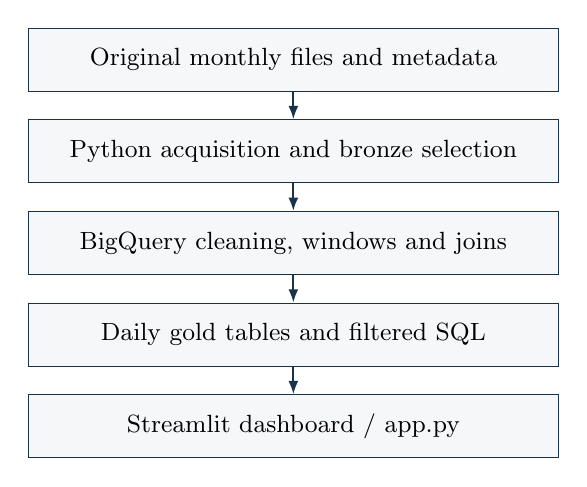
\begin{tikzpicture}[node distance=3.5mm,box/.style={draw=navy,fill=navy!4,text width=6.5cm,minimum height=8mm,align=center,font=\small},arr/.style={-{Latex[length=1.7mm]},thick,navy}]
\node[box] (a) {Original monthly files and metadata};
\node[box,below=of a] (b) {Python acquisition and bronze selection};
\node[box,below=of b] (c) {BigQuery cleaning, windows and joins};
\node[box,below=of c] (d) {Daily gold tables and filtered SQL};
\node[box,below=of d] (e) {Streamlit dashboard / app.py};
\draw[arr](a)--(b);\draw[arr](b)--(c);\draw[arr](c)--(d);\draw[arr](d)--(e);
\end{tikzpicture}
\end{column}
\begin{column}{.41\textwidth}
\textbf{Quality and provenance}\par
Checksums and row reconciliation. IST dates with unique UTC keys. No missing-value filling.
\medskip

\textbf{Independent check}\par
DuckDB reference outputs verify cloud results. It is a validation path.
\medskip

\textbf{Application access}\par
Read-only viewer credentials, bound parameters and a ten-minute cache.
\end{column}\end{columns}
\end{frame}

\begin{frame}{4. Pollutant Rules and Combined Pollution Level}
\begin{center}\begin{tabular}{lll}\toprule
Pollutant & Reference & Daily comparison\\\midrule
PM2.5 / PM10 & 60 / 100 $\mu$g/m$^3$ & 24-hour mean\\
NO2 / SO2 & 80 / 80 $\mu$g/m$^3$ & 24-hour mean\\
NH3 & 400 $\mu$g/m$^3$ & 24-hour mean\\
O3 & 100 $\mu$g/m$^3$ & Highest eligible 8-hour mean\\
CO & 2 mg/m$^3$ & Highest eligible 8-hour mean\\\bottomrule
\end{tabular}\end{center}
\begin{itemize}
\item Each day needs at least 16 valid hourly observations.
\item An 8-hour window needs six readings and stays within the IST day.
\item Combined level: worst available CPCB band, from 0 Good to 5 Severe.
\item Require at least three valid pollutants, including PM2.5 or PM10 [2].
\end{itemize}
\begin{block}{Interpretation}
The combined measure is an ordinal screening level, not official numeric AQI. Missing pollutants can hide a worse band. O3 upper bands use the source table's one-hour convention.
\end{block}
\end{frame}

\begin{frame}{5. Coverage and Persistent Hotspot Detection}
\begin{columns}[T]
\begin{column}{.48\textwidth}
\textbf{Coverage}\[
100\times\frac{\text{valid observed days}}{\text{calendar days in period}}
\]
\textbf{High-day fraction}\[
100\times\frac{\text{high days}}{\text{valid observed days}}
\]
Missing days never count as clean days.
\end{column}
\begin{column}{.48\textwidth}
\textbf{Default persistence rule}
\begin{itemize}\setlength\itemsep{2mm}
\item Overall day coverage at least 75\%.
\item Each counted month also has at least 75\% coverage.
\item At least 10\% high days in each counted month.
\item At least three high-pollution months.
\end{itemize}
\end{column}\end{columns}
\medskip
\begin{block}{Transparent project choices}
Thresholds are adjustable. PM2.5 persistent counts change from 370 at 60\% coverage to 342 at 75\% and 250 at 90\%. This changes eligibility, not the measured air quality.
\end{block}
\end{frame}

\begin{frame}{6. Dashboard Output: Pollution Hotspots}
\centering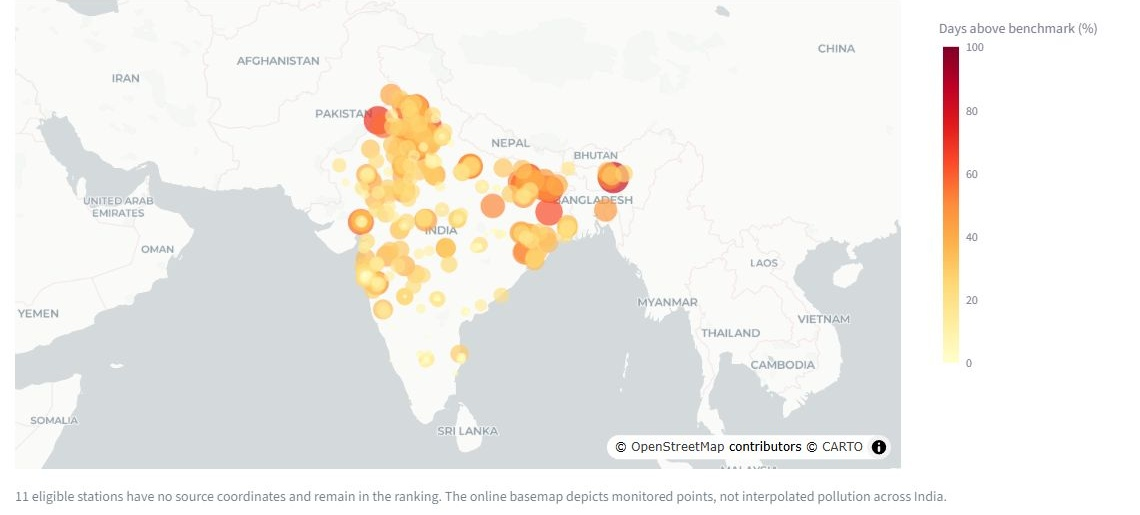
\includegraphics[width=.90\linewidth,height=.59\textheight,keepaspectratio]{../assets/dashboard_map.jpg}
\begin{itemize}
\item PM2.5 default view: 416 coverage-eligible stations, 342 persistent.
\item Sector-51, Gurugram: 84.2\% high days from 330 valid days.
\item Eleven eligible stations lack coordinates and remain in the ranking.
\end{itemize}
\end{frame}

\begin{frame}{7. Dashboard Output: Monthly Patterns}
\centering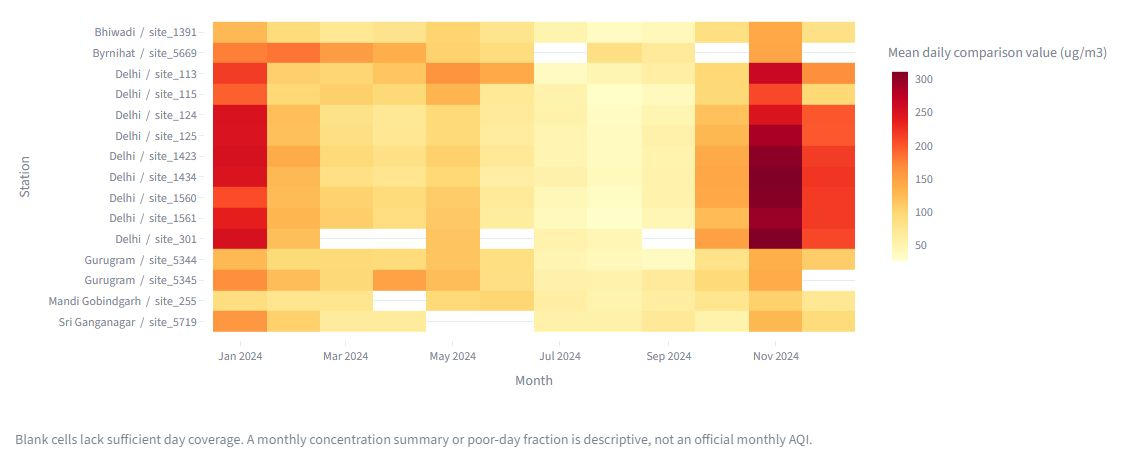
\includegraphics[width=.98\linewidth,height=.62\textheight,keepaspectratio]{../assets/dashboard_monthly.jpg}
\begin{itemize}
\item Means of daily PM2.5 values for the top 15 ranked stations.
\item Blank cells fall below the coverage rule. A second heatmap shows coverage.
\item One year describes monthly differences, not recurring seasonality or causes.
\end{itemize}
\end{frame}

\begin{frame}{8. Dashboard Output: Combined Level and Comparison}
\textbf{432 coverage-eligible stations and 222 persistent hotspots}\par
\centering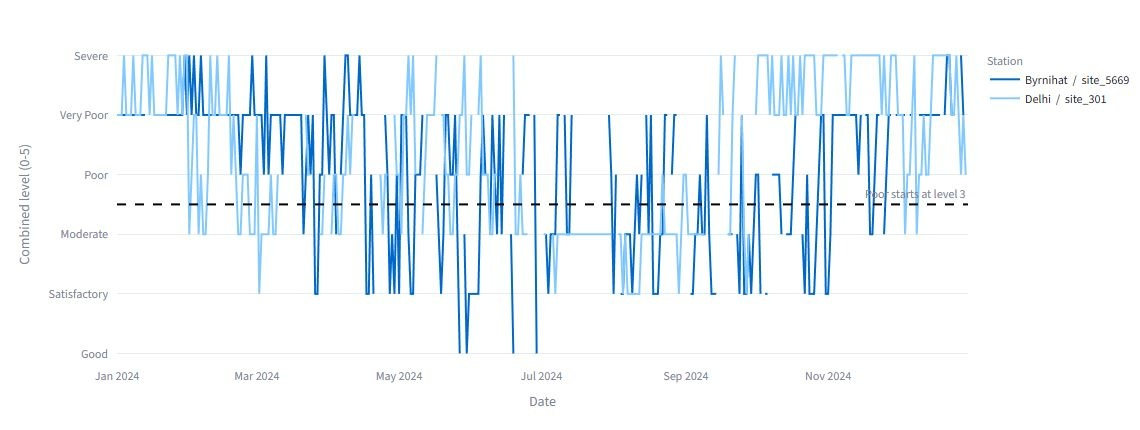
\includegraphics[width=.98\linewidth,height=.65\textheight,keepaspectratio]{../assets/dashboard_combined_plot.jpg}
\begin{itemize}
\item Derived combined level from 0 Good to 5 Severe. Poor starts at level 3.
\item Daily details show available pollutants. Compare up to three stations and export CSV.
\end{itemize}
\end{frame}

\begin{frame}{9. Results, Validation and Course Alignment}
\begin{columns}[T]
\begin{column}{.45\textwidth}
\textbf{Default annual screening}\par\medskip
\begin{tabular}{lrr}\toprule
View & Eligible & Persistent\\\midrule
PM2.5 & 416 & 342\\
PM10 & 412 & 372\\
NO2 & 425 & 35\\
SO2 & 432 & 4\\
O3 & 421 & 167\\
CO & 435 & 172\\
NH3 & 389 & 0\\\bottomrule
\end{tabular}
\end{column}
\begin{column}{.51\textwidth}
\textbf{Validation evidence}
\begin{itemize}
\item 32 tests passed after cleanup.
\item Four cloud output tables match the local reference.
\item Three dashboard aggregation scenarios match.
\end{itemize}
\medskip
\textbf{ED547 connection}\par
Modules IV and V: ETL, Google BigQuery, SQL and Python. Modules I and II: lifecycle, data quality and warehouse storage.
\end{column}\end{columns}
\begin{block}{Verified execution}
Retained job IDs and processed-byte records establish real BigQuery execution. Hadoop, Spark and Airflow are not implemented. No controlled speed benchmark is claimed.
\end{block}
\end{frame}

\begin{frame}{10. Conclusion, Limitations and References}
\textbf{Conclusion}\par
The project links large-scale cloud processing to station-level evidence, coverage-aware persistence and reproducible outputs.\par
\medskip
\textbf{Limitations}
\begin{itemize}
\item Historical 2024 data only. No prediction or attribution of causes.
\item Uneven monitoring, missing pollutants and 53 missing-coordinate stations.
\item Derived combined level and adjustable project thresholds.
\item Sandbox tables expire after 60 days. Internet and credentials are required [3].
\end{itemize}
\medskip
\textbf{References}\par\scriptsize
[1] XKDR Forum. India Air Quality Database. \url{https://airquality.xkdr.org/}\par
[2] Indian Economic Service. National Air Quality Index.\par
\url{https://ies.gov.in/arthapedia/concept/national-air-quality-index}\par
[3] Google Cloud. BigQuery sandbox. \url{https://docs.cloud.google.com/bigquery/docs/sandbox}\par
\vspace{1mm}Accessed 1 November 2026. Results: retained project audits and analytical exports.
\end{frame}
\end{document}
